\chapter{Descrição e desenvolvimento do projeto}


    Neste capítulo são apresentados o desenvolvimento da proposta e também sua implementação no FlexA e a documentação produzida. Inicialmente será apresentado o que foi alterado da estrutura atual do FlexA para que o projeto proposto pudesse ser executado, e após isso as alterações feitas no modelo de comunicação e segurança serão mostradas, e por fim serão debatidas as técnicas utilizadas na implementação da versão móvel do FlexA.


    \section{Adaptação do modelo desenvolvimento do FlexA}

        A versão atual do FlexA não possuí um modelo de programação bem definido, com pouca documentação e a inexistência de uma convenção do fluxo de dados dentro do sistema. Carente também de uma padronização explicita da transmissão dos metadados.
        
        Dessa forma um estudo mais a fundo do sistema foi realizado, utilizando a pouca documentação que existia do sistema e a análise de todo o código-fonte, para entender o real funcionamento e comportamento do sistema, e como era definida a estrutura atual do projeto. Após esse estudo foi criado um diagrama para representar o estado atual dos módulos do sistema, e suas dependências conforme pode ser visto na Figura \ref{fig:pacotesMario}.
        
        \begin{figure}
            \centering
            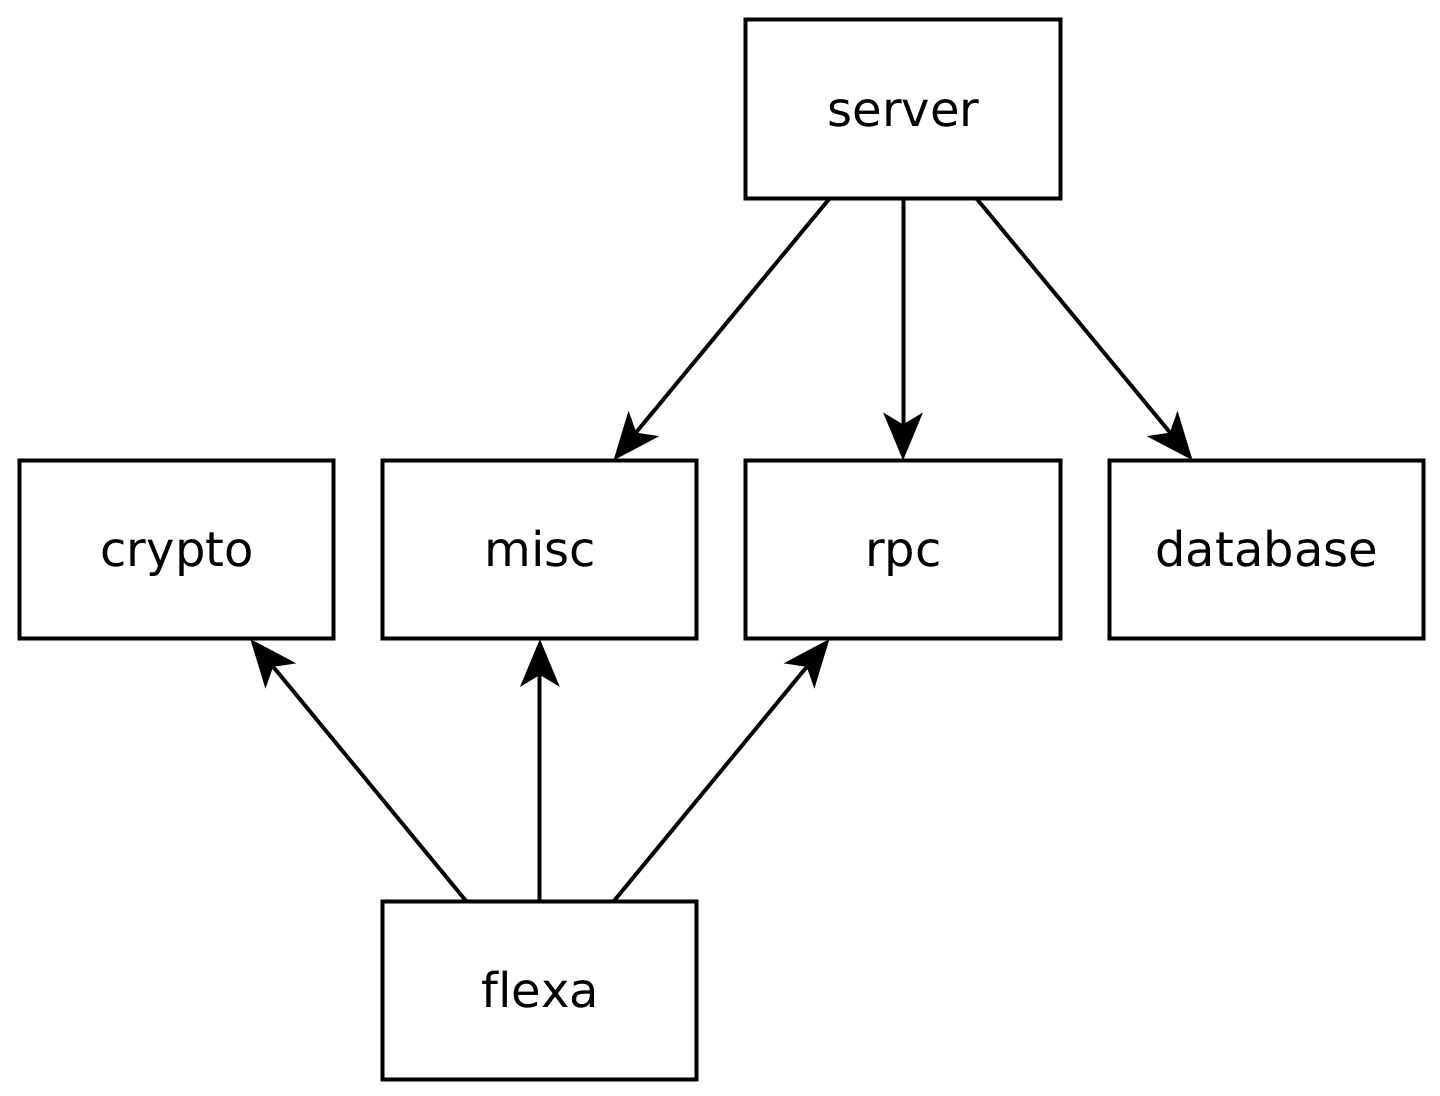
\includegraphics[width=10cm]{pacotesMario.png}
            \caption{Módulos do sistema atual e suas dependências. ~\cite{mario}.}
            \label{fig:pacotesMario}
        \end{figure}
        
        Esse diagrama foi gerado a partir do estudo do código-fonte da versão atual do projeto. Apenas por esse diagrama já é possível notar que o módulo Servidor em momento algum utiliza os serviços de criptografia, e que apenas o servidor tem acesso aos bancos de dados de metadados.
        
        Além do diagrama de módulos do sistema também foi criado um diagrama de classes, para que fosse possível analisar a estrutura mais interna dos módulos. Esse diagrama é apresentado na figura \ref{fig:classesMario}. Embora seja um diagrama de classes, alguns abusos de notação tiveram que ser utilizados devido a lacuna existente entre a representação dos diagramas de Classes da Unified Language Model (UML)~\cite{umlClasses} e a linguagem Python em que o FlexA é desenvolvido.
        
        \begin{figure}[!ht]
        \centering
        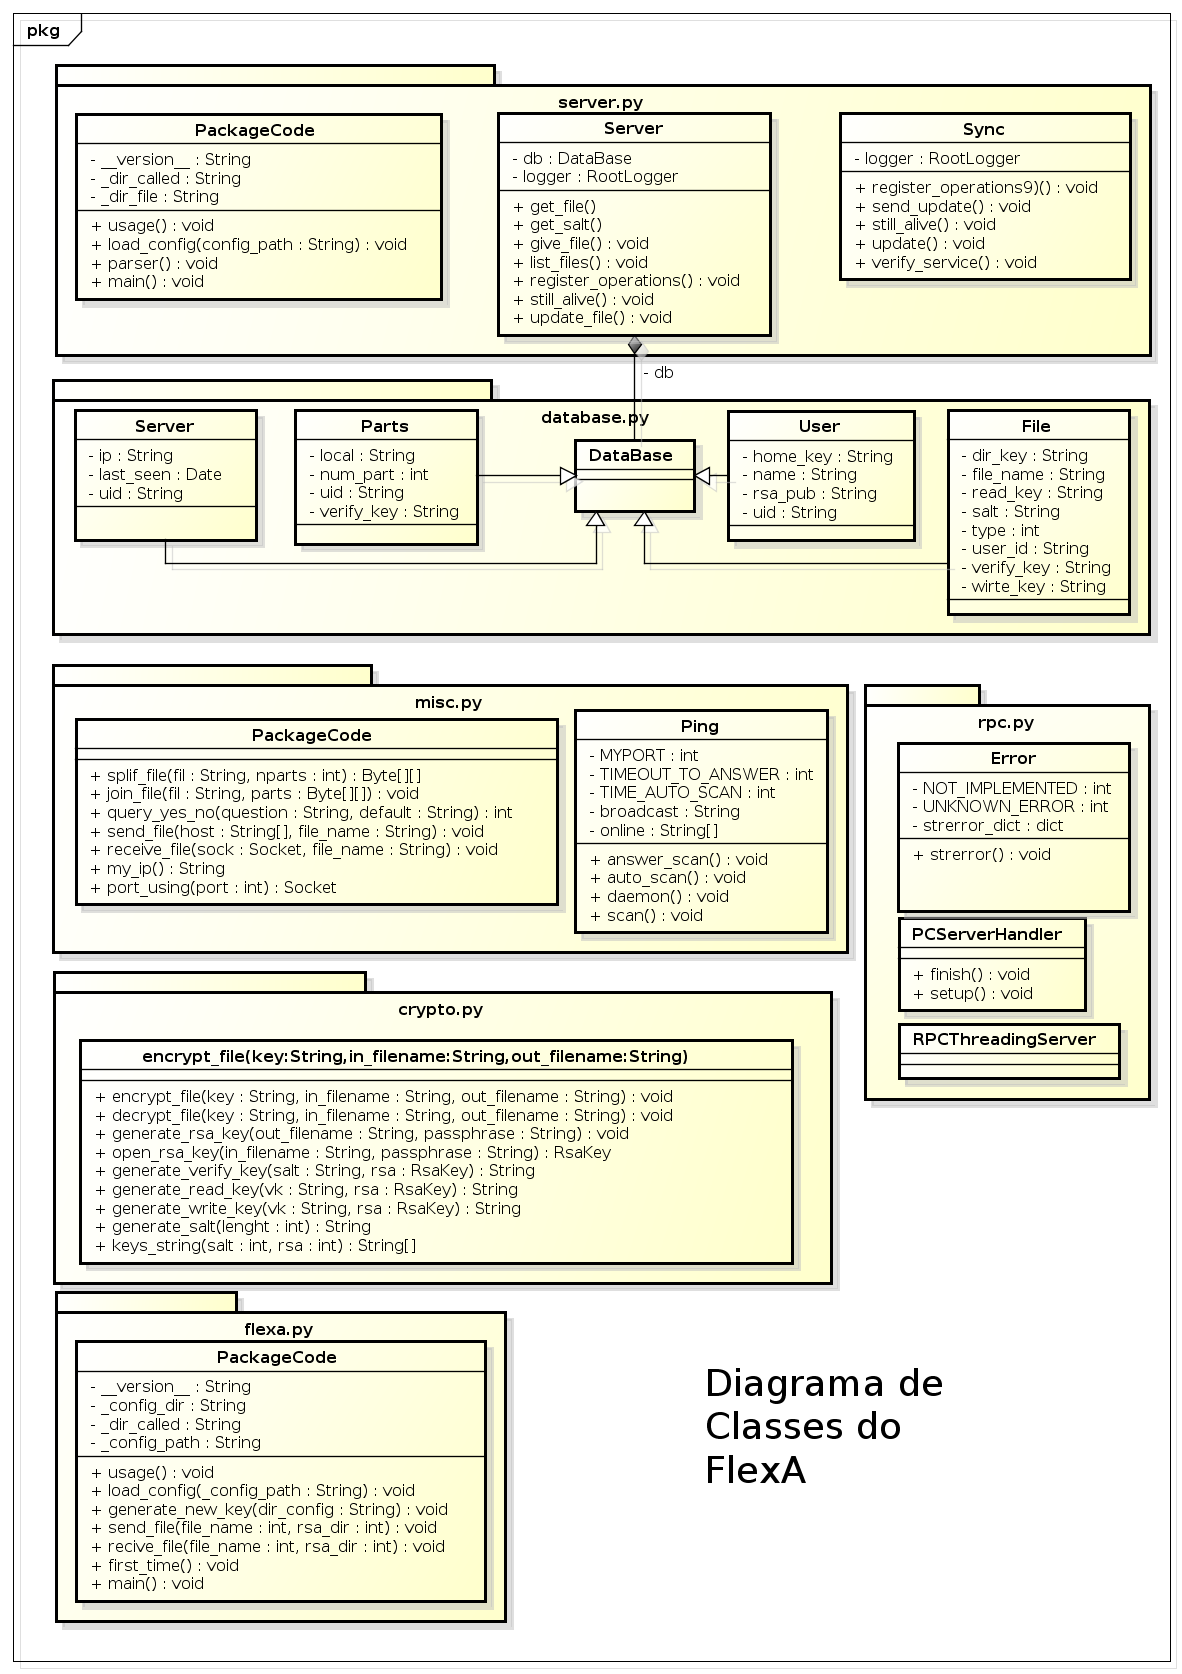
\includegraphics[width=14cm]{classesMario.png}
        \caption{Classes e pacotes (arquivos) que estruturam a versão atual do FlexA}
        \label{fig:classesMario}
        \end{figure}
             

        Analisando o diagrama de classes apresentado na Figura \ref{fig:classesMario} é possível perceber que muitas atividades diferentes e classes distintas pertencem a um mesmo pacote. Até esse trabalho, como todo o FlexA era desenvolvido apenas em Python, não havia problema em manter o padrão de desenvolvimento atual. 
        
        Conforme a proposta desse trabalho, desenvolver um cliente para Android do FlexA e melhorar os quesitos de abertura do FlexA, se mostrou necessário realizar alterações no projeto para que fosse possível a execução desses objetivos.
        
        Em um primeiro momento foi feito o levantamento dos requisitos do FlexA, junto com os objetivos de melhoria do código existente. Dessa forma foi elaborado o seguinte diagrama UML de casos de uso de acordo com ~\cite{umlCasosDeUso}. O diagrama com os casos de uso é apresentado na Figura \ref{fig:casosDeUsoGabriel}.
        
        \begin{figure}
        %
        %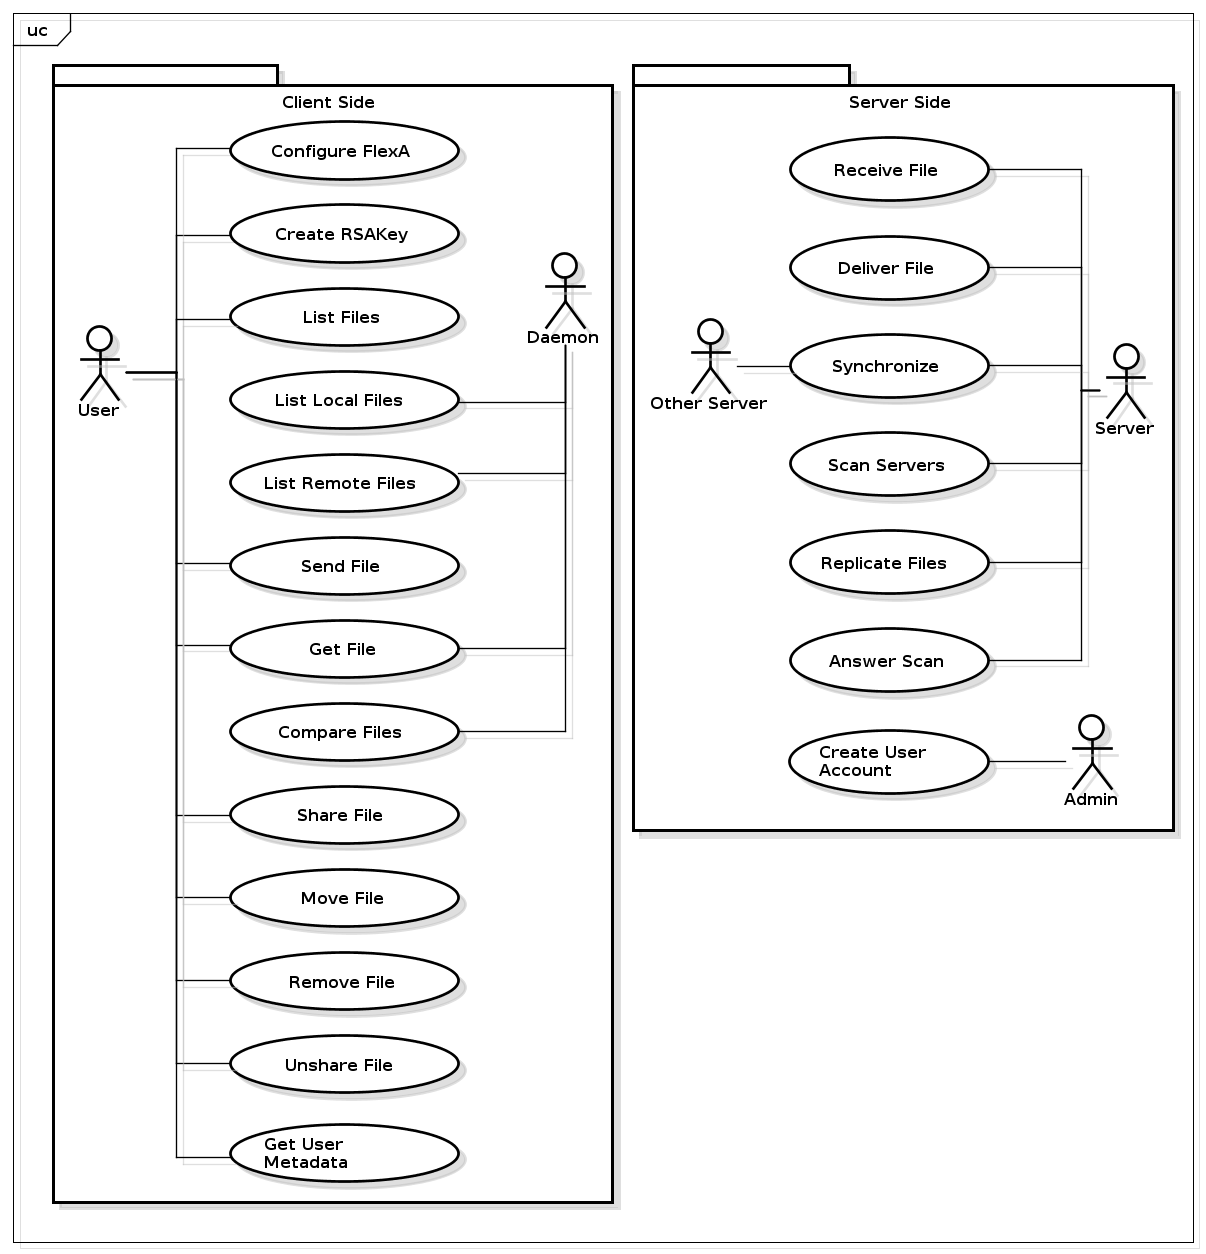
\includegraphics[width=15cm]{casosDeUsoGabriel.png}
        %\caption{Diagrama de Casos de uso com os requisitos funcionais do FlexA.}
        \label{fig:casosDeUsoGabriel}
        \end{figure}
    
        Uma vez definidas quais são as funcionalidades que são esperadas do sistema, iniciou-se uma analise mais profunda das comunicações entre cliente e servidor. Poucas informações foram encontradas em ~\cite{mario} e ~\cite{silas} sobre a padronização da comunicação entre cliente e servidores, e o pouco que foi encontrado já estava defasado devido a grandes alterações no sistema desde então. Dessa forma foi necessário analisar o código fonte e entender exatamente como eram feitas as comunicações nas diversas operações existem.
        
        
        
        
        
        
        
        Após o estudo da comunicação entre cliente e servidor ~\cite{mario} formalizou-se, utilizando a notação para protocolos de comunicação apresentada em ~\cite{ross} que é mostrada na tabela \ref{tab:notacao}:
        
        \begin{table}
        
        \centering
        \begin{tabular}{|l|l|}
        \hline
        
        $C$ & módulo cliente ou usuário \\
        \hline
        $S$ & módulo servidor \\
        \hline
        $privKey_{X}$ & chave privada $X$ \\
        \hline
        $pubKey_{X}$ & chave pública $X$ correspondente a $privKey_{X}$\\
        \hline
        $C \rightarrow S : dado$ & $C$ envia $dado$ para $S$\\
        \hline
        $C \rightarrow S : {dado}_{pubKey_{x}}$ & $C$ envia $dado$ criptografado com a chave pública $X$ para $S$\\
        \hline
        
        \end{tabular}
        \caption{Notação utilizada para definição de protocolos de comunicação ~\cite{ross}.}
        \label{tab:notacao}
        \end{table}
        
        Feito as definições que serão utilizadas a seguir, são apresentados os protocolos para as comunicações. Esses protocolos foram elaborados baseados no código fonte ~\cite{mario} já inserindo as adaptações para fornecer maior compatibilidade e segurança ao sistema.





        
        A primeira formalização é o protocolo para solicitação dos metadados do usuário que acaba de iniciar o FlexA pela primeira vez ou quando seja necessário obter seu \textit{userID}. Isso é feito com base em sua chave pública previamente cadastrada no sistema por um administrador. O protocolo é apresentado na figura \ref{fig:proMetadadosUsuario}.
        
        \begin{figure}
        
        \[ C \rightarrow S: pubKey_{C} \]
        \[ S \rightarrow C: \{userID, homeKey\}_{pubKey_{C}} \]
        
        \caption{Protocolo de requisição dos metadados de um usuário com base na sua chave}
        \label{fig:proMetadadosUsuario}
        \end{figure}
        
        Com os metadados do usuário (\textit{userID} e \textit{homeKey} que é o identificador se sua pasta raiz) o usuário pode começar a utilizar o sistema enviando e recebendo arquivos.
        
        Para que o usuário possa enviar um arquivo para o sistema é necessário verificar se existe um arquivo com o mesmo nome no mesmo endereço. Caso o arquivo não existe ainda, é feito o cadastro e solicitado o \textit{salt} referente ao arquivo. Na figura \ref{fig:proGetSalt} é formalizado o protocolo de requisição do \textit{salt} de um arquivo. É importante ressaltar que \textit{fileName} é composto pelo nome completo do arquivo com o diretório em que o arquivo se encontra. Esse nome é relativo ao diretório mapeado do FlexA para o usuário referenciado por \textit{userID}.

        \begin{figure}
        \[ C \rightarrow S: fileName,userID \]
        \[ S \rightarrow C: salt \]
        \caption{Requisição do \textit{salt} de um arquivo}
        \label{fig:proGetSalt}
        \end{figure}
        
        Caso o \textit{salt} retornado pelo servidor seja igual $0$ é definido assumido que esse arquivo ainda não existe no servidor com esse nome.
        
        Já com o \textit{salt}, o módulo cliente gera o trio de chaves para o arquivo (VK, RK e WK), criptografa o arquivo utilizando a RK, faz a divisão do arquivo e envia cada porção para um servidor. Para enviar as porções aos servidores o módulo cliente faz primeiro o cadastro do arquivo no servidor e então envia as porções. Na figura \ref{fig:proSendFile} é descrito o protocolo para essa ação, onde $N$ é o número de porções em que o arquivo foi dividido, $dirKey$ é o identificador do diretório que o arquivo está e $fileType$ é o tipo do arquivo (diretório ou arquivo comum).
        
        \begin{figure}
        
        Para i de 1 até N:
        \[ C \rightarrow S_{i}: fileName,(VK,WK),dirKey,userID,fileType \]
        \[ S_{i} \rightarrow C: port \]
        
        
        \caption{Cadastro do arquivo nos servidores e negociação da porta de envio do arquivo}
        \label{fig:proSendFile}
        \end{figure}
        
        Após o cadastro do arquivo e a negociação da porta de transmissão do arquivo, é feita a transmissão do arquivo em uma nova conexão com o servidor na porta $port$.
        
        Com a negociação pronta basta enviar para o servidor a porção correspondente. Essa comunicação é definida conforme o protocolo mostrado na figura \ref{fig:proSendFileData}.
        
        \begin{figure}
        Para i de 1 até N:
        \[ C \rightarrow S_{i}: filePart_{i} \]

        \caption{Transmissão das porções dos arquivos aos $N$ servidores}
        \label{fig:proSendFileData}
        \end{figure}
        
        
        Com os protocolos já definidos é possível enviar um arquivo para o servidor. Mas ainda não é possível recuperar os arquivos enviados. Agora serão tratados os protocolos envolvidos na recuperação dos arquivos enviados aos servidores.
        
        Para recuperar um arquivo, é de grande importância a capacidade de listar os arquivos de um diretorio. Para essa ação de listar arquivos é utilizado o protocolo da figura \ref{fig:proListFiles}.
        
        \begin{figure}
        \[ C \rightarrow S:  \]
        \[ C \rightarrow S_{i}: filePart_{i} \]

        \caption{Transmissão das porções dos arquivos aos $N$ servidores}
        \label{fig:proListFiles}
        \end{figure}
        
        
        
        
        
        
        
        
        
        
        
        
        
        